% Native TikZ source. Incidence drawing, not a circle packing.
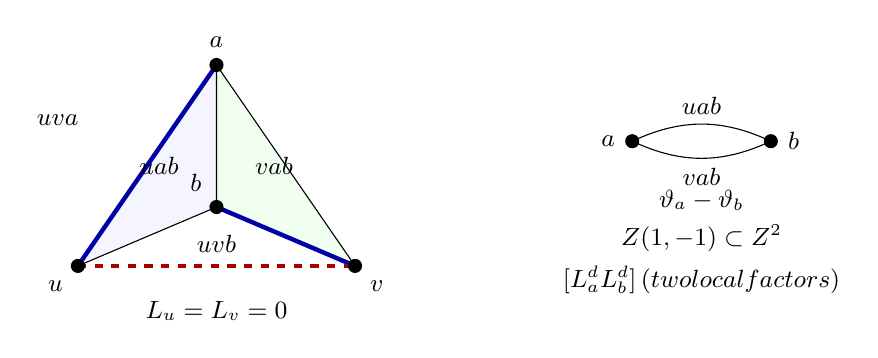
\begin{tikzpicture}[scale=.88, every node/.style={font=\small},
  vertex/.style={circle,fill=black,inner sep=1.8pt},
  matching/.style={draw=blue!65!black,line width=1.6pt},
  marked/.style={draw=red!65!black,dashed,line width=1.2pt}]
  \coordinate (u) at (-2,0);
  \coordinate (v) at (2,0);
  \coordinate (a) at (0,2.9);
  \coordinate (b) at (0,.85);
  \fill[blue!4] (u)--(a)--(b)--cycle;
  \fill[green!6] (v)--(a)--(b)--cycle;
  \draw[matching] (u)--(a);
  \draw[matching] (v)--(b);
  \draw[marked] (u)--(v);
  \draw (u)--(b)--(a)--(v);
  \node[vertex,label=below left:$u$] at (u) {};
  \node[vertex,label=below right:$v$] at (v) {};
  \node[vertex,label=above:$a$] at (a) {};
  \node[vertex,label=above left:$b$] at (b) {};
  \node at (-.83,1.45) {$uab$};
  \node at (.83,1.45) {$vab$};
  \node at (0,.32) {$uvb$};
  \node[anchor=east] at (-1.85,2.1) {$uva$};
  \node at (0,-.65) {$L_u=L_v=0$};
  \begin{scope}[xshift=7cm]
    \coordinate (aa) at (-1,1.8);
    \coordinate (bb) at (1,1.8);
    \draw (aa) to[bend left=25] node[above] {$uab$} (bb);
    \draw (aa) to[bend right=25] node[below] {$vab$} (bb);
    \node[vertex,label=left:$a$] at (aa) {};
    \node[vertex,label=right:$b$] at (bb) {};
    \node[align=center] at (0,.65)
      {$\vartheta_a-\vartheta_b$\\[3pt]$\mathbb Z(1,-1)\subset\mathbb Z^2$};
    \node at (0,-.2) {$[L_a^dL_b^d]\,(\text{two local factors})$};
  \end{scope}
\end{tikzpicture}
